\chapter{Fast Fourier sampling for dummies}\label{chap:ffs}


\section{Introduction}

\subsection{Roadmap}

\section{Preliminaries}\label{sec:ffs:prelim}

% \subsection{Rings and matrices over Rings}
% 
% Let $\phi \in \bR[x]$ be a monic polynomial with distinct roots over $\bC$, $\cR = \bR[x]/(\phi(x))$ be a polynomial quotient ring and $a,b$ be arbitrary elements of $\cR$. 
% \begin{itemize}
%  \item 
%  We note $\adj{a}$ and call (Hermitian) adjoint of $a$ the unique element of $\cR$ such that for any root $\zeta$ of $\phi$, $\adj{a}(\zeta) = \overline{a(\zeta)}$, where $\overline{\cdot}$ is the usual complex conjugation over $\bC$. We can extend this definition to matrices: the adjoint of a matrix $\matB \in \cR^{n\times m}$ is the coefficient-wise adjoint of the transpose of $\matB$.
%  \item
%  The inner product over $\cR$ is $ \inner{a}{b} = \frac{1}{\deg(\phi)}\sum_{\phi(\zeta)=0} a(\zeta)\cdot \overline{b(\zeta)} = \frac{1}{\deg(\phi)} \fft(a) \cdot \adj{\fft(b)}$, and the associated norm is $\|a\| = \sqrt{\inner{a}{a}}$. This definition extends to vectors $\veca,\vecb$ of $\cR^m$: $\inner{\veca}{\vecb} = \sum_i \inner{a_i}{b_i}$.
% \end{itemize}
% The reason of the presence of the scaling factor $\frac{1}{\deg(\phi)}$ in the definition of the inner product is to make it coincide with the usual coefficient dot product $\inner{a}{b}_2 = \sum_i a_i b_i$ in useful cases: when $\phi(x) = x^n \pm 1$, $\inner{a}{b} = \inner{a}{b}_2 $ for any $a,b \in \bR[x]/(\phi(x))$. However, we note that in general the inner product $\inner{\cdot}{\cdot}$ and the coefficient dot product $\inner{\cdot}{\cdot}_2$ (resp. the norm $\|\cdot\|$
% and the coefficient norm $\|\cdot\|_2$) do not coincide. This difference is not inocuous, and in \falcon{} we systematically use the inner product $\inner{\cdot}{\cdot}$ and its associated norm $\|\cdot\|$, unless stated otherwise.

\paragraph{Linearization operators: a first attempt.} For a polynomial ring $\cR = \bR[x]/(\phi(x))$ of extension degree $d=\deg(\phi)$ over $\bR$, it is often convenient to represent vectors of $\cR^m$ (resp. matrices of $\cR^{m\times n}$) as vectors of $\bR^{md}$ (resp. matrices of $\bR^{md\times nd}$). We lose the ring structure, but in exchange some useful operations (such as orthogonalization) can be done at a fainer-grained level. For vectors of $\cR^m$, this can be done simply by applying the \fft{} component-wise -- which we note $\fft(\vecv)$. For matrices, we define the linear map $\cC : \cR^{n\times m} \rightarrow \bC^{dn \times dm}$ as follows. First, for any $a\in \cR$, the circulant matrix of $a$ is
 
 \begin{equation}
\cC(a) = \begin{bmatrix*}[c]   \fft(a) \\
\fft(xa) \\
 \vdots \\
\fft(x^{d-1}a) \\ \end{bmatrix*} \in \bC^{d\times d}.
\end{equation}
This definition generalizes to matrices by component-wise application. One can check that for any vector $\vecv$ and matrices $\matB,\matC$ such that the products $\vecv \matB$ and $\matB \matC$ are defined, the map $\cC$ satisfy the following properties: 
\begin{enumerate}
 \item 
 $\cC$ is an injective algebra morphism. In particular, $\cC(\matB) \cC(\matC) = \cC(\matB \matC)$.
 \item\label{item:circ}
 $\fft(\vecv)\cC(\matB) = \fft(\vecv \matB)$.
\end{enumerate}

The second point illustrates that the maps $\fft$ and $\cC$ are complementary. Indeed, for $a\in \cR$, the $\fft$ maps $a$ to its unique decomposition according to a basis $(e_1,\dots,e_{\deg(\phi)})$. For the same basis, $\cC(a)$ is the transformation matrix of the injective map $f \in \cR \mapsto f a$. This is the intrinsic reason that makes these two properties valid. In addition, $\cC$ allows to easily compute the inner product of elements $x^i a, x^j b\in\cR$: indeed, $\cC(a) \times \adj{\cC(b)} = (\inner{x^i a}{x^j b})_{i,j}$

One can intuitively see why the map $\fft$ and $\cC$ may not be optimal: they interpret $\cR$ (resp. the algebra $\text{End}(\cR)$ of endomorphisms of $\cR$) as a $\bR$-module of dimension $\deg(d)$, without accounting for potential additional structure, like the fact that $\cR$ may belong to a tower of rings. In section~\ref{sec:ffs:prelim:klein}, we will show that this is a limitation of the maps $\fft$ and $\cC$ when using Klein's sampler. In Section~\ref{sec:ffs:prelim:cyclo}, we will define maps $\Ve,\Ma$ analogous to $\fft,\cC$ but which truly exploit tower of rings structures.



\subsection{Gram-Schmidt orthogonalization and the LDL decomposition}\label{sec:ffs:prelim:gso}

% \paragraph{Full-rank matrices.}
% Let $\matB \in \cR^{n \times m}$. We say that $\matB$ is full-rank (or is a basis) if for any linear combination $ \sum a_i \vecb_i$ with $a_i \in \cR$, we have the equivalence $(\sum_i a_i \vecb_i = \veczero) \Longleftrightarrow (\forall i, a_i = 0)$.
% 
% We note that since $\cR$ is generally not an integral domain, a set formed of a single nonzero vector is not necessarily full-rank. In the rest of the paper, a basis will either denote a set of independent vectors $\{\vecb_1,\ldots\vecb_n\} \in (\cR^m)^n$, or the full-rank matrix $\matB \in \cR^{n \times m}$ whose rows are the $\vecb_i$'s.
% 
% We say that a self-adjoint matrix $\matG \in \cR^{n \times n}$ is full-rank Gram if there exist $m \geq n$ and a full-rank matrix $\matB \in \cR^{n \times m}$ such that $\matG = \matB \adj\matB$. This generalizes the notion of positive definiteness for symmetric real matrices.

\paragraph{The Gram-Schmidt orthogonalization.}
Any matrix $\matB \in \cR^{n \times m}$ can be decomposed as follows:
\begin{equation}
 \matB = \matL \times \tBB,
\end{equation}
where $\matL$ is lower triangular with only $1$'s on the diagonal, and the rows $\tBB$ are pairwise orthogonal. When $\matB$ is full-rank , this decomposition is unique, and it is called the Gram-Schmidt orthogonalization.
We will also call Gram-Schmidt norm of $\matB$ the following value:
\begin{equation}
 \gsnorm{\matB} = \max_{\tilde\vecb_i \in \tBB} \|\tilde\vecb_i\|.
\end{equation}

\paragraph{The $\LDLs$ decomposition.} Closely related to the Gram-Schmidt orthogonalization is the Gram-Shmidt decomposition. The $\LDLs$ decomposition writes any full-rank Gram matrix as a product $\L \matD \adj\L$, where $\matL \in \cR^{n\times n}$ is lower triangular with $1$'s on the diagonal, and $\matD \in \cR^{n\times n}$ is diagonal. It can be computed using algorithm~\ref{alg:ldl}.

%  \begin{algorithm}
%  \caption{$\ldlalgo(\matG)$}\label{alg:ldl}
%  \begin{algorithmic}[1]
%  \Require {A full-rank Gram matrix $\matG = (G_{ij}) \in \cR^{n\times n}$.}
%  \Ensure {The decomposition $\matG = \L \matD \adj\L$ over $\cR$, where $\L$ is unit lower triangular and $\matD$ is diagonal.}
%  \State{$\L, \matD \gets \matzero^{\ n\times n}$}
%  \For{$i$ from $1$ to $n$}
%  \State{$\l_{ii} \gets 1$}
%  \State {$D_{i} \gets G_{ii} - \sum_{j<i} \l_{ij} \adj \l_{ij} D_j$}
%  \For{$j$ from $1$ to $i-1$}
%  \State {$\l_{ij} \gets \frac{1}{D_{j}} \left( G_{ij} -  \sum_{k<j} \l_{ik} \adj \l_{jk} D_k \right)$}
%  \EndFor 
%  \EndFor
%  \Return{$((\l_{ij}),\Diag_i(D_i))$}
%  \end{algorithmic}
%  \end{algorithm}

 The $\LDLs$ decomposition and the \gso{} are closely related as for a basis $\matB$, there exists a unique \gso{} $\matB = \L \cdot \tBB$ and for an FRG matrix $\matG$, there exists a unique $\LDLs$ decomposition $\matG = \L  \matD  \adj\L$. If $\matG = \matB \adj \matB$, then $\matG = \L \cdot (\tBB \adj \tBB) \cdot \adj\L$ is a valid $\LDLs$ decomposition of $\matG$. As both decompositions are unique, the matrices $\L$ in both cases are actually the same. In a nutshell:
\begin{equation}
 \left[\L\cdot\tBB \text{ is the \gso{} of } \matB \right]
  \Leftrightarrow  \left[ \L \cdot (\tBB\adj \tBB) \cdot \adj\L  \text{ is the $\LDLs$ decomposition of }(\matB\adj \matB)\right].
\end{equation}
The reason why we present both equivalent decompositions is because the \gso{} allows to provide a more intuitive explanation of Klein's sampler, whereas the use of $\LDLs$ decomposition is faster and therefore makes more sense from an algorithmic point of view.

\subsection{Klein's sampler}\label{sec:ffs:prelim:klein}


Klein's sampler is historically the first trapdoor sampler. Its existence actually predates the very concept of trapdoor sampling, since it was first used in a different context~\cite{SODA:Klein00}. It is defined for lattices over $\bR^m$ and is described in algorithm~\ref{alg:klein}.

 \begin{algorithm}[H]
 \caption{$\klein(\vect, \L, \matD, \sigma)$}
 \label{alg:klein}
 \begin{algorithmic}[1]
 \Require { The $\LDLt$ decomposition $\matB \matB^\t  = \L \cdot \matD \cdot \L^\t$ for $\matB\in \bR^{n\times m}$, a vector $\vect \in \bR^n$}
 \Ensure { A vector $\vecz \in \bZ^n$ such that $\vecz \cdot \matB \sim D_{\Lambda(\matB), \sigma, \vect \matB}$}
 \For{$j = n,\ldots,1$}
 \State{$\bar{t}_j \gets  t_j + \sum_{i>j} (t_i - z_i) \l_{ij}$}
 \State{$\sigma_j \gets \sigma/\sqrt{D_{jj}}$}
 \State{$z_j \gets \gaussround{\bar{t}_j}{\sigma_i}$}
 \EndFor                                                                                                             
 \Return{$\vecz$}
  \end{algorithmic}
 \end{algorithm}
 Klein's sampler is a randomized version of the nearest plane algorithm~\cite{STACS:Babai85,Combinatorica:Babai86}. The latter is deterministic and outputs vectors in $[-1,1]^m \cdot \matB$. In Klein's sampler, the rounding at each step $j$ is replaced by a discretized Gaussian of parameter $\sigma_j = \sigma/\|\tilde\vecb_j\|$. It has been shown that if $\sigma \geq \smooth(\bZ^m) \cdot \gsnorm{\matB}$ for a suitable $\epsilon$, then $\klein(\vect, \L, \matD, \sigma) \cdot \matB$ is statistically close to the ideal Gaussian oracle $D_{\Lambda(\matB), \sigma, \vect \matB}$ under various metrics of closeness: the statistical distance~\cite{AC:DucNgu12a}, the Kullback-Leibler divergence~\cite{AC:DucLyuPre14} or the R\'enyi divergence~\cite{AC:Prest17}. This is illustrated by the figure~\ref{fig:nptoklein}.
 
 
 \begin{figure}[H]
 \centering
$\begin{array}{ccc}
 \fbox{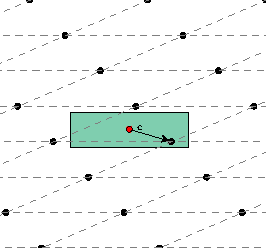
\includegraphics{tikz/BabaiNP}}  &\Longrightarrow& \fbox{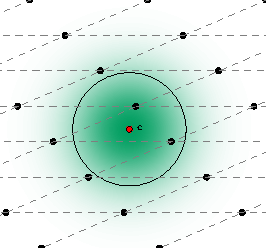
\includegraphics{tikz/Klein}} \\
 \text{Nearest plane algorithm} & & \text{Klein's sampler} \\
\end{array}$
\caption{From the nearest plane algorithm to Klein's sampler.}\label{fig:nptoklein}
\end{figure}
 

Klein's sampler works only with matrices having coefficients in $\bR$. If we are to work in a ring $\cR = \bR[x]/(x^d\pm 1)$ instead, a straightforward approach to use it while preserving its good security properties is to interpret $\cR$ as a $\bR$-module of dimension $d$. This is done by replacing the vector $\vect \in \cR^{n}$ with $c(\vect)$, and the matrices $\matB, \matB \adj\matB$ with the block circulant matrices $\cC(\matB), \cC(\matB \adj\matB)$.

The problem with this approach is that this interpretation of $\cR$ as a $\bR$-module completely breaks the ring structure that $\cR$ enjoys. As a consequence, the $\LDLs$ decomposition has no obvious structure that Klein's sampler could exploit: its total complexity becomes $O(n^2d^2)$.
 

% \subsection{Cyclotomic rings}\label{sec:ffs:prelim:cyclo}
% This section gives a few reminders about cyclotomic polynomials and rings, especially for the rings of interests in the \falcon{} scheme. For $d \in \bN^\star$, $\zeta_d$ denotes an arbitrary primitive $d$-th root of unity in $\bC$, for example $\zeta_d = e^{\frac{2i\pi}{d}}$. We may note $\Omega_d = \{\zeta_d^k | k \in\bZ_d^\times \}$ the set of primitive $d$-th roots of unity. Let
% \begin{equation}
% \phi_d(x) = \prod\limits_{\zeta \in \Omega_d} (x - \zeta) = \prod\limits_{k\in\bZ_d^\times} (x - \zeta_d^k). 
% \end{equation}
% 
% This polynomial is in $\bZ[x]$ and is called the $d$-th cyclotomic polynomial.
% It is immediate that for any $d$, the degree of $\phi_d$ is $\varphi(d)$, where $\varphi(d) = |\bZ_d^\times|$ is Euler's totient function. For special values of $d$, the cyclotomic polynomial $\phi_d$ is easy to compute:
% \begin{itemize}
%  \item If $d=2^k$ for $k \geq 1$, then $\phi_d(x) = \phi_2(x^{d/2}) = x^{d/2}+1$.
% %  \item If $d=2^k \cdot 3^\ell$ for $k \geq 1$ and $\ell \geq 2$, then $\phi_d = \phi_{18}(x^{d/18}) = x^{d/3} - x^{d/6} + 1$.
% \end{itemize}
% We will also note $\cR_d = \bR[x]/(\phi_d)$ and $\cZ_d = \bZ[x]/(\phi_d)$.
% 
% \paragraph{Switching between representations.} For any cyclotomic ring $\bR[x]/(\phi_d)$ and any element $f = \sum_{i=0}^{\phi(d)-1} f_i x^i \in \bR[x]/(\phi_d)$, one may easily switch between the representation $\vecf = (f_i)_{0\leq i< \varphi(d)}$ of $f$ in the coefficient embedding and its representation $\hat\vecf = (f(\zeta))_{\{\phi_d(\zeta)=0\}}$ in the canonical embedding via the fast Fourier transform which, when $d$ is highly composite, can be computed in time $O(d \log d)$.
% 
% Another noteworthy property is that for the cases which interest us, computing $\inner{f}{g}$ from $\vecf,\vecg$ and $\inner{f}{g}_2$ from $\hat\vecf,\hat\vecg$ can be done in time $O(d)$ without having to perform any (inverse) fast Fourier transform.
% Indeed, $\hat\vecf = \vecf\cdot \matV_d$, where $\matV_d$ is a Vandermonde matrix: $\matV_d = (\zeta_d^{ij})_{\{0 \leq i < \phi(d), j \in \bZ_d^\times\}}$. Therefore:
% \begin{itemize}
%  \item $\inner{f}{g} = \frac{1}{\phi(d)} \hat\vecf \cdot \hat\vecg^\star = \frac{1}{\phi(d)} \vecf \cdot \matV \times \adj{\matV} \cdot \adj\vecg$.
%  \item $\inner{f}{g}_2 = \vecf \cdot \vecg^\t = \hat\vecf \cdot (\matV \times \adj{\matV})^{-1} \cdot \hat\vecg^{-\star}$.
% \end{itemize}
% For the values of $d$ used in \falcon{}, $\matV_d \times \adj\matV_d $ can be expressed simply:
% \begin{itemize}
%  \item If $d=2^k$ for $k \geq 1$, then $\matV_d \times \adj\matV_d = \phi(d) \matI_{\phi(d)}$.
%  \item If $d=2^k \cdot 3^\ell$ for $k \geq 1$ and $\ell \geq 2$, then we have $\matV_d \times \adj\matV_d = \phi(d) \left[ \matI_{\phi(d)} + \frac{1}{2} \matJ_{\phi(d)}\right]$ and $(\matV_d \times \adj\matV_d )^{-1} = \frac{4}{3\phi(d)} \left[ \matI_{\phi(d)} - \frac{1}{2} \matJ_{\phi(d)}\right]$, for $\matJ_n = \twotwo{\matzero_{n/2}}{\matI_{n/2}}{\matI_{n/2}}{\matzero_{n/2}}$.
% \end{itemize}
% 
% 
% These are the only properties which are needed in \falcon{}. For additional documentation about cyclotomic polynomials, rings and fields, the readers can refer to e.g.~\cite{Lang95}, Chapter IV.
%  
% % \subsection{Linearization operators}\label{sec:ffs:prelim:lin}
% 
% TODO:
% \begin{itemize}
%  \item Interpretation: $\Ve$ is a natural way of breaking down the ring $\cR_d$ into a product of smaller rings. It is an isomorphism, so for $\Ve: \cR_d \rightarrow \cR_{d'}^k$ we have that $\cR_{d'}^k$ is itself a ring with the operations induced by this isomorphism: for $\vecx, \vecy \in \cR_{d'}^k$, $\vecx \vecy = \Ve( \Ve^{-1}(\vecx) \Ve^{-1}(\vecy) )$.
%  \item + example for power of two cyclotomics
%  \item $\Ma$ writes the transformation matrix of the map $f \mapsto fa$
% \end{itemize}
% 
% \paragraph{Tower of rings.} A convenient fact about cyclotomic polynomials is that they can often be envisioned as parts of tower of rings. We make the following observation:
% \begin{itemize}
% \item
% Any cyclotomic ring $\bR[x]/(\phi_{2d}(x))$ lives as a subring of  $\bR[y]/(\phi_{4d}(y))$ via the morphism $x \mapsto y^2$
% % \item
% % Any cyclotomic ring $\cR = \bR[x]/(\phi(x))$ -- in particular $\bR[x]/(\phi_{18}(x))$ -- can be viewed as a $\bR$-linear space of dimension $\deg(\phi)$ via the morphism $f \in \cR \mapsto \fft(f) \in \bC^{\deg(\phi)}$.
% \end{itemize}
% 
% From this, it follows that the base rings used in \falcon{} sit atop tower of rings as decribed below:
% \begin{itemize}
% \item
% For $\lambda = 128$: $\bR = \cR_2 \subsetneq \cR_4 \subsetneq \cR_8 \subsetneq \cR_{16} \subsetneq \cR_{32} \subsetneq \cR_{64} \subsetneq \cR_{128} \subsetneq \cR_{256} \subsetneq \cR_{512}$.
% % \item
% % For $\lambda = 192$: $\bR = \cR_2 \subsetneq \cR_{18} \subsetneq \cR_{36} \subsetneq \cR_{72} \subsetneq \cR_{144} \subsetneq \cR_{288} \subsetneq \cR_{576} \subsetneq \cR_{1152} \subsetneq \cR_{2304}$.
% \item
% For $\lambda = 256$: $\bR = \cR_2 \subsetneq \cR_4 \subsetneq \cR_8 \subsetneq \cR_{16} \subsetneq \cR_{32} \subsetneq \cR_{64} \subsetneq \cR_{128} \subsetneq \cR_{256} \subsetneq \cR_{512} \subsetneq \cR_{1024}$.
% \end{itemize}
% 
% Now, the next step is to devise linearization operators similar to the $\fft$ and $\cC$. Unlike the $\fft$ (resp. $\cC$) which directly maps $\cR = \bR[x]/(\phi(x))$ (resp. $\text{End}(\cR)$) to $\bC^{\deg\phi}$, these maps procede in a more gradual way by allowing to decompose $\cR$ over intermediate rings $\cR'$ such that $\bR \subsetneq \cR' \subsetneq \cR$.
% 
% \paragraph{The linearization operators $\Ve$ and $\Ma$.}
% Let $d,d'\in \bN^\star$ such that $d'$ divides $d$ strictly (noted $d'|d$). We define the ring-splitting maps $\V{d}{d'}:\cR_d^m \rightarrow \cR_{d'}^{md/d'}$ and $\M{d}{d'} : \cR_d^{n\times m} \rightarrow \cR_{d'}^{(nd/d') \times (md/d')}$ by induction as follows:
% \begin{itemize}
% \item
% If $d$ is a multiple of $4$ and $d'=d/2$, let $a$ be an arbitrary element of $\cR_d$. $a$ can be uniquely decomposed as $a(x) = a_0(x^2) + x a_1(x^2)$, with $a_0, a_1 \in \cR_{d'}$. We then define $\V{d}{d'}(a) = (a_0,a_1)$ and
% \begin{equation}
% \M{d}{d'}(a) = \twotwo{a_0}{a_1}{y a_1}{a_0} = \twoone{\V{d}{d'}(a)}{\V{d}{d'}(xa)}.
% \end{equation}
% % \item
% % If $d$ is a multiple of $2$ but not of $4$ and $d'=2$, then we fall back to the ``classical'' maps $\fft,\cC$: $\V{d}{d'}(a) = \fft(a)$ and $\M{d}{d'}(a) = \cC(a)$.
% \item 
% We extend the definition of $\V{d}{d'}$ (resp. $\M{d}{d'}$) to vectors (resp. matrices) by component-wise application.
% \item
% For $d''|d'|d$, we define $\V{d}{d''}$ and $\M{d'}{d''}$ by induction:
% \begin{equation}
%  \V{d}{d''} = \V{d'}{d''} \circ \V{d}{d'} \text{ and } \M{d}{d''} = \M{d'}{d''} \circ \M{d}{d'}.
% \end{equation}
% 
% \end{itemize}
% When clear from context, we may omit $d,d'$ in the notations as explained hereinafter. For $\vecv \in \cR_{d}^m$ and $\matB \in \cR_{d}^{n\times m}$, we note $\Ve(\vecv) = \V{d}{(d/2)}(\vecv)$ (resp. $\Ma(\matB) = \M{d}{(d/2)}(\matB)$).
% % , where $d'$ is the largest value for which $\V{d}{d'}(\vecv)$ (resp. $\M{d}{d'}(\matB)$) is defined (which is either $d/2$ or $2$).
% In our algorithms, we will use $\Ve$ and $\Ma$ as often as possible, as they allow to ``gently'' descent down tower of rings.
% 
% 
% \section{Preprocessing the basis: Fast Fourier orthogonalization}\label{sec:ffs:ffo}
% 
% Our goal is now to use the linearization operators $\Ve,\Ma$ 
% 
%  \begin{algorithm}[H]
%  \caption{$\ffldl(\matG)$}\label{alg:ffldl}
%  \begin{algorithmic}[1]
%  \Require {A full-rank Gram matrix $\matG \in \cR_{d}^{n\times n}$}
%  \Ensure {\small The compact $\LDLt$ decomposition of $\matG$ in FFT form}
%  \State {$(\L,\matD) \leftarrow \ldlalgo(\matG)$}\label{step:ldl}
%   \If{$d=2$}
%  \Return{$(\L,\matD)$}
%  \EndIf
%  \For{$i=1,\ldots,n$}
%  \State {$\tL_i \leftarrow \ffldl(\Ma(\matD_{ii}))$}\label{step:ffldl}
%  \EndFor
%  \Return $(\L, (\tL_i)_{1\leq i\leq n})$
%  \end{algorithmic}
%  \end{algorithm}
%  
% \section{Trapdoor sampling: the Fast Fourier sampler}\label{sec:ffs:ffs}
% 
% 
% % TODO:
% % \begin{itemize}
% %  \item Many, many things
% %  \item handle precision issues
% %  \item R\'enyi argument
% % \end{itemize}
% 
%  \begin{algorithm}[H]
%   \caption{$\ffklein_{\cR_d}(\vect, \tL, \sigma)$}\label{alg:ffnp}
%  \begin{algorithmic}[1]
%   \Require {$\vect \in \cR_d^n$, a precomputed tree $\tL$, (implicitly) a matrix $\matB \in \cR_d^{n \times m}$ such that $\tL$ is the compact $\LDLt$ decomposition tree of $\matB\adj \matB$.}
%   \Ensure {$\vecz \in \cZ_d^n$ such that $\vecz \cdot \matB \sim D_{\Lambda(\matB), \sigma, \vect \matB}$.}
%   \If{$d=2$}\label{step:bottom1}
%   \State $(\matL, \matD) \gets \tL $
%   \Return{$\klein(\vect, \L, \matD, \sigma)$}\label{step:bottom2}
%   \EndIf\label{step:bottom3}
%  \State{$(\L, (\tL_i)_{1\leq j\leq n}) \leftarrow \tL$}
%  \For{$j = n,\ldots,1$}
%  \State{$\btt_j \leftarrow  \vect_j + \sum_{i>j} (\vect_i - \vecz_i) \l_{ij}$}\label{step:np}
%  \State{$\vecz_j \leftarrow \Ve^{-1} \left[\ffklein( \Ve(\btt_j), \tL_j, \sigma) \right]$}\label{step:ffnp}
%  \EndFor                                                                                                             
%  \Return{$ \vecz = (\vecz_i,\dots,\vecz_n)$}
%   \end{algorithmic}
%  \end{algorithm}
%  
%  \paragraph{Indistinguishability from an ideal Gaussian.} If $\sigma \geq \smooth(\bZ) \cdot \gsnorm{\matB}$, then the ratio between the distribution $\ffklein_{\cR_d}(\vect, \tL, \sigma) \cdot \matB$ and the ideal Gaussian is always between $\left(\frac{1-\epsilon}{1+\epsilon}\right)^{n \varphi(d)}$ and $\left(\frac{1-\epsilon}{1+\epsilon}\right)^{n \varphi(d)}$. This can be shown by applying inductively the original proof from~\cite{STOC:GenPeiVai08}. The relative error between the two is therefore bounded by approximately $2n \varphi(d) \epsilon $. Following the security arguments from \cite[Section 3.3]{AC:Prest17}, as long as:
%  \begin{equation}
%  \epsilon \leq \frac{1}{n \varphi(d) \sqrt{\lambda q_s}},
%  \end{equation}
% we can replace the ideal Gaussian with the fast Fourier sampler and it will make \falcon{} lose at most one bit of security.